%%
%%  Department of Electrical, Electronic and Computer Engineering.
%%  EPR400/2 Final Report - Section 2.
%%  Copyright (C) 2011-2021 University of Pretoria.
%%

\section{Approach}
The aim of this project was to develop a system that would track and  illuminate mosquitoes with a laser. The system will detect mosquitoes using a camera and laser will be controlled by a turret system. The system is implicitly required to operate in real-time in order to track and illuminate mosquitoes with a laser. This was taken into consideration in all the design aspects of the system. The project entails the first principles design of the following:
\begin{itemize}
      \item A laser turret that can change the position of a laser beam.
      \item A control system that can control the laser turret.
      \item An object detection algorithm that can detect mosquitoes.
      \item An object detection algorithm that can detect the reflections of the laser beam.
      \item A multi-target tracking algorithm that can track multiple mosquitoes and predict their future locations.
\end{itemize}

The laser turret was inspired by two-axis laser scanners that use two mirrors to direct a laser beam in two dimensions as illustrated in \autoref{fig:two-axis-scanner-schematic}. The advantages of this approach compared to moving that laser diode itself is that the mirrors are rotated about their centre of mass which reduces the torque required to rotate the mirrors. This enables the laser turret to rapidly change the position of the mirrors and in tern the position of the laser beam. The drawback of this approach is that there will be additional scattering of the laser beam due to imperfections in the mirrors. This will not have significant impact on the system, therefore, this approach was chosen for the laser turret. A closed-loop \gls{pid} control system will be used to control the laser turret. The laser position feedback for the control system will be provided by the laser detection system.

The object detection algorithm to detect mosquitoes can be implemented using a deep learning approach that will enable the identification and appearance matching of mosquitoes. This approach is computationally expensive and will require quality high-resolution images of mosquitoes. A less computational expensive approach is to use image segmentation techniques to separate the mosquitoes from the background of the image. An image segmentation approach greatly reduces the computational complexity at the expense of flexibility and robustness. Another trade-off to consider is that this approach will not be able to distinguish between mosquitoes and other objects similar in appearance. Image segmentation does not require the same quality and resolution images as a deep learning approach since it will not distinguish between objects of similar appearance. The benefits of an image segmentation approach outweigh the trade-offs compared to a deep learning approach for this project. Therefore, the image segmentation approach was chosen for this project.

The same considerations were made for the object detection algorithm to detect the reflections of the laser beam. An image segmentation approach was chosen for the same reasons as discussed above.

The multi-target tracking algorithm is required to track and predict the locations of mosquitoes. This can be efficiently achieved using a Kalman filter for one object. The Kalman filter is a recursive algorithm that can be used to estimate the state of a system that is subject to random noise. The Kalman filter is able to recursively predict the future state of a system, which is required to predict the future locations of a mosquito. This can be extended to track multiple objects using the \gls{sort} algorithm that combines the Kalman filter and the Hungarian algorithm. The Hungarian algorithm is an optimal assignment algorithm that can be used to assign detections to tracks. The \gls{sort} algorithm is less computationally complex than other multi-target tracking algorithms while maintaining a comparable or higher accuracy \cite{SORT-Bewley2017}.

A high-level overview of the system can be seen in \autoref{fig:system_overview}. The system was designed to operate in a controlled environment.
\begin{figure}[h]
      \centering
      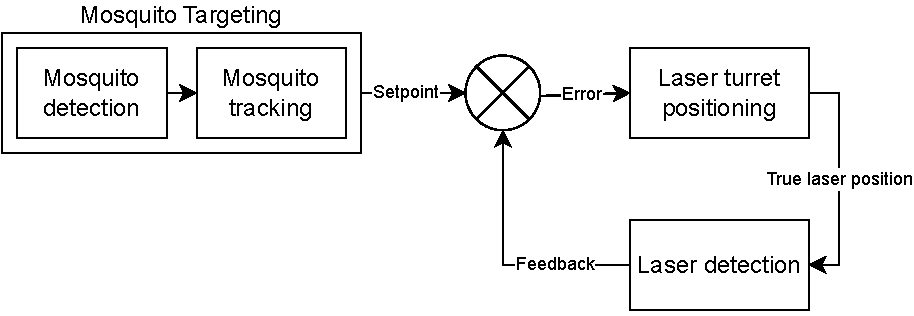
\includegraphics[width=1\textwidth]{figures/system_overview.pdf}
      \caption{Overview of the system.}
      \label{fig:system_overview}
\end{figure}

\newpage

%% End of File.

